\documentclass[12pt]{article}

\usepackage[table]{xcolor}

\usepackage[hidelinks]{hyperref}
\usepackage{etoolbox}
\usepackage{graphicx}
\usepackage{adjustbox}

\makeatletter
\def\ScaleIfNeeded{%
  \ifdim\Gin@nat@width>\linewidth
    \linewidth
  \else
    \Gin@nat@width
  \fi
}
\makeatother

% fonts
\usepackage[T1]{fontenc}
\usepackage[utf8]{inputenc}
\usepackage{textgreek}
\usepackage[greek,english]{babel}
\usepackage{amsmath}

% Code highlight and colors
\usepackage{listings}
\lstset{
  numbers=left,
  tabsize=1,
  basicstyle=\small\ttfamily,
  breaklines=true
}

\usepackage{booktabs, tabularx, longtable}
\usepackage{csquotes}
\usepackage{authblk}

% Geometry block
\usepackage[letterpaper]{geometry}
\providecommand{\tightlist}{\setlength{\itemsep}{0pt}\setlength{\parskip}{0pt}}

\title{Interactions retain the co-phylogenetic matching that communities lost}

\author[1,2,3]{Timothée~Poisot}
\author[1]{Daniel B.~Stouffer}
\affil[1]{Centre for Integrative Ecology, School of Biological Sciences,
University of Canterbury, Christchurch, New Zealand}
\affil[2]{Université de Montréal, Département de Sciences Biologiques, Montréal,
Canada}
\affil[3]{Québec Centre for Biodiversity Sciences, Montréal, Canada}

\begin{document}

\maketitle

\begin{abstract}
  Both species and their interactions are affected by changes that occur
  at evolutionary time-scales, and these changes shape both ecological
  communities and their phylogenetic structure. That said, extant
  ecological community structure is contingent upon random chance,
  environmental filters, and local effects. It is therefore unclear how
  much ecological signal local communities should retain. Here we show
  that, in a host--parasite system where species interactions vary
  substantially over a continental gradient, the ecological significance
  of individual interactions is maintained across different scales.
  Notably, this occurs despite the fact that observed community variation
  at the local scale frequently tends to weaken or remove community-wide
  phylogenetic signal. When considered in terms of the interplay between
  community ecology and coevolutionary theory, our results demonstrate
  that individual interactions are capable and indeed likely to show a
  consistent signature of past evolutionary history even when woven into
  communities that do not.
\end{abstract}

% pandoc-xnos: macro to create a caption without a prefix
\makeatletter
\long\def\@makenoprefixcaption#1#2{
  \vskip\abovecaptionskip
  \sbox\@tempboxa{#2}
  \ifdim \wd\@tempboxa >\hsize
    #2\par
  \else
    \global \@minipagefalse
    \hb@xt@\hsize{\hfil\box\@tempboxa\hfil}
  \fi
  \vskip\belowcaptionskip}
\makeatother

% pandoc-fignos: save original macros
\makeatletter
\let\@oldmakecaption=\@makecaption
\let\oldthefigure=\thefigure
\let\oldtheHfigure=\theHfigure
\makeatother

% pandoc-fignos: environment disables figure caption prefixes
\makeatletter
\newcounter{figno}
\newenvironment{no-prefix-figure-caption}{
  \let\@makecaption=\@makenoprefixcaption
  \renewcommand\thefigure{x.\thefigno}
  \renewcommand\theHfigure{x.\thefigno}
  \stepcounter{figno}
}{
  \let\thefigure=\oldthefigure
  \let\theHfigure=\oldtheHfigure
  \let\@makecaption=\@oldmakecaption
  \addtocounter{figure}{-1}
}
\makeatother

% pandoc-xnos: cleveref fakery
\newcommand{\plusnamesingular}{}
\newcommand{\starnamesingular}{}
\newcommand{\xrefname}[1]{\protect\renewcommand{\plusnamesingular}{#1}}
\newcommand{\Xrefname}[1]{\protect\renewcommand{\starnamesingular}{#1}}
\providecommand{\cref}{\plusnamesingular~\ref}
\providecommand{\Cref}{\starnamesingular~\ref}
\providecommand{\crefformat}[2]{}
\providecommand{\Crefformat}[2]{}

% pandoc-xnos: cleveref formatting
\crefformat{figure}{fig.~#2#1#3}
\Crefformat{figure}{Figure~#2#1#3}
\crefformat{table}{table~#2#1#3}
\Crefformat{table}{Table~#2#1#3}
\crefformat{equation}{eq.~#2#1#3}
\Crefformat{equation}{Equation~#2#1#3}

Ecological interactions often exert important selective pressures on the
species involved. For example, the phenologies of lodgepole pines and
red crossbills respond spatially to the presence of squirrels (Benkman
et al. 2003). Likewise, palm species undergo changes in seed morphology
in response to the extinction of birds dispersing their seeds (Galetti
et al. 2013; Johnson et al. 2017). Interactions can be lost, too, when
phenologies of the species involved shift (Rafferty et al. 2015).
Interactions are, in fact, so important that the existence of a species
has been inferred by the fact that another species bore traits that
matched no other known species: Kritsky (1991) relates the discovery of
the moth \emph{Xanthopan morganii}, with a proboscis famously over a
foot long, which Darwin predicted would exist based solely on the
phenology of local plant \emph{Angraecum sesquipedale}. In addition,
interactions and the emergent structures they define are distributed in
similar ways across communities at both large or small scales (Jordano
et al. 2003). Together, these observations suggest that much ecological
structure could be the end result of (co)evolutionary dynamics between
species (Eklöf et al. 2012; Stouffer et al. 2012). Unfortunately,
although the evolutionary dynamics of pairs of interacting species have
been well described at macro-evolutionary (Van Valen 1973) and
micro-evolutionary (Gandon et al. 2008) timescales, most attempts to
understand how they cascade up to the levels of diversity of both
species and interactions found within empirical communities have been
inconclusive (Hembry et al. 2014). This suggests that these
well-describe mechanisms may not confer substantial predictive power
when examined at scales of organization larger than the pairwise
interaction.

Historically, the evidence for shared evolutionary history in
taxonomically diverse communities relied on the quantification of the
degree of matching between the phylogenies of two sets of interacting
organisms, accounting for the distributions of interactions across the
phylogeny (Legendre et al. 2002). This notion builds on the century-old
idea that extant species interact in a way similar to the way their
ancestors did (Fahrenholz 1913; Guimarães Jr et al. 2011; Nuismer et al.
2013). Note that testing these assumptions is related to, but markedly
more restrictive than, testing for phylogenetic conservatism of species'
interactions (Rezende et al. 2007; Eklöf et al. 2012). This is because
of additional, higher-order constraints related to the shape of both
trees at \emph{all} depths (Cavender-Bares et al. 2009; Mouquet et al.
2012), because ancestral evolutionary innovations have a high
phylogenetic inertia, and they carry forward to extant taxa (Desdevises
et al. 2003; Diniz-Filho \& Bini 2008; Vale \& Little 2010). In a way,
the true measure of phylogenetic signal of interactions should depend
not only on how they are conserved within the tree of the species
establishing them (\emph{e.g.} parasites or pollinators), but also how
these interactions at matched to the tree of the species receiving them
(\emph{e.g.} hosts or plants). This is true whether or not the species
complex are coevolving: in fact, neutral interactions can yield
perfectly matching co-phylogenies (Poisot 2015). Consequently, many of
the systems that have been described as exhibiting significant
phylogenetic structure of interactions ultimately deviate from this last
constraint, and this can occur for a variety of factors that stem from
how other species evolved and established, lost, or maintained
interactions throughout their joint evolutionary history. Nonetheless,
detecting matching phylogenies for interacting clades indicates that
their shared evolutionary history is long standing and is therefore
suggestive that their extant ecological structure is an outcome of
ancestral constraints and/or co-adaptation (Nuismer \& Harmon 2015).

It is important to note further that discovering matching phylogenies
does not mean that coevolutionary dynamics---\emph{sensu} Thompson
(1999)---took place at any time. In fact, coevolution is not expected to
necessarily result in matching phylogenies nor are matching phylogenies
only produced through coevolution (Poisot 2015). It follows that
community-level measures of phylogenetic signal, while they \emph{do}
quantify how closely interactions are a product of phylogeny, do not
allow us to draw conclusions on coevolution. Nevertheless,
interaction-level measures are useful, in that, when expressed as the
contribution of interactions to the overall signal, they allow us to
\emph{compare} the importance of interactions across replicated
communities. Communities from the same regional pool vary because (i)
the local species pool is at best a subset of the regional species pool
and (ii) the local interactions are at best a subset of the interactions
in the regional community (Poisot et al. 2015). This implies that (i)
the phylogenetic signal in the regional pool will be different from the
signal in the local communities, and (ii) the phylogenetic signal across
local communities will differ. Species sampling and variability of
interactions, however, does no predict (i) how the phylogenetic signal
of pairwise interactions is kept or lost at the scale of the whole
community nor (ii) whether or not this variability is related to changes
in the amount of phylogenetic signal that can be detected locally.

In this manuscript, we analyze a large dataset of over 300 species of
mammalian hosts and their ectoparasites, sampled throughout Eurasia, for
which phylogenetic relationships are known. Using a Procrustean approach
to quantify the strength of co-phylogenetic matching of interactions
between host and parasite trees (Balbuena et al. 2013), we show that
locally sampled communities rarely show strong matching despite the fact
that the overall system does at the continental scale. We then provide
evidence to support the conclusion that the amount of phylogenetic
matching within a local community is predictable based on the importance
of interactions in the regional network. We finally show that the
contribution of specific interactions to phylogenetic matching is
invariant across scales, and is unrelated to their tendency to vary
across space. The lack of co-phylogenetic structure in local communities
suggests that, while interactions are undeniably important for community
assembly, they might be less so than abiotic factors.

\section{Methods}\label{methods}

\subsection{Data source and
pre-treatment}\label{data-source-and-pre-treatment}

We use data on observations of interactions between 121 species of
rodents and 205 species of parasitic fleas in 51 locations across Europe
(Krasnov et al. 2012b) to build 51 species-species interaction networks.
Interactions were measured by combing rodents for fleas, a method that
gives high quality data as it has a high power of detection. The dataset
also includes phylogenies for the hosts and the parasites. Previous
analyses revealed that this dataset shows significant co-phylogenetic
matching at the continental level (Krasnov et al. 2012a). Importantly,
it also provides spatial replication and variability (Canard et al.
2014) at a scale large enough to capture macro-ecological processes.
This dataset is thus uniquely suited for our analysis as it represents a
thorough spatial and taxonomic sampling of a paradigmatic system in
which interspecific interactions are thought to be driven by
macro-evolution and co-speciation events (Combes 2001; Verneau et al.
2009).

The original dataset gives quantitative interaction strengths (expressed
as an averaged number of parasites per species per host). In this
system, quantitative interaction strengths were previously shown to be
affected to a very high degree by local variations in abundance across
sampling locations (Canard et al. 2014), and it therefore seems unlikely
that they reflect macro-ecological processes. Therefore, to account for
differential sampling effort---which cannot readily be quantified---and
across site variations in abundance---which do not pertain to
macro-evolutionary processes---we only study the networks' bipartite
incidence matrices (that is, presence and absence of infection of hosts
by the parasites).

\subsection{Spatial scales and interaction spatial
consistency}\label{spatial-scales-and-interaction-spatial-consistency}

Noting that variation of interactions across locations---which can be
caused by local ecological mechanisms as opposed to reflecting
evolutionary dynamics---can decrease congruence, we analyze the data at
three different levels which we will refer to as continental, regional,
and local. Notably, the continental level summarizes the complete
dataset whereas both the regional and local levels are location-specific
scales.

\emph{Continental} interaction data consists of the aggregated
\enquote{metanetwork} which includes all documented interactions between
species from the regional species pool (Poisot et al. 2012). For every
location, we further define two scales of analysis.

First, \emph{regional} interaction data accounts for different species
composition across sites: the species that have been observed locally
interact as they would do in the \emph{continental} network, \emph{i.e.}
if interactions did not vary across space. This allows testing whether
sampling from the regional species pool affects co-phylogenetic
matching, regardless of the distribution of interactions. Within each
site, the regional scale is given by the subset of the metanetwork
formed by the locally present species (properly speaking, the induced
subgraph of the metanetwork induced from the nodes of the local
network). Hence the regional networks are always a perfect subset of the
continental network, and do not reflect whether species were actually
observed to interact locally or not, but whether they \emph{can}
interact at all. This \emph{regional} network is thus a baseline
estimate derived from interactions within the species pool and measures
the effect of species sampling on co-phylogenetic matching.

Second, \emph{local} interaction data are the actual observations at
this location: the identity of the present species, and the way they
interact. In addition to capturing the dissimilarity of species
composition across sites, this allows measuring the effect of
interaction turnover across space. The local and regional networks
always include the same species, but the local network has only a subset
(or, at most, an exact match) of the interactions in the regional
network.

We finally define the spatial consistency of every interaction as the
proportion of sites in which the two co-occurring species interact with
each other, or simply

\begin{equation} S_{ij} = \frac{L_{ij}}{C_{ij}}\,. \label{eq:linktunover}\end{equation}

The spatial consistency of an interaction \(S_{ij}\) between species
\(i\) and \(j\) is therefore the ratio between the the number of
locations in which they were observed to interact (\(L_{ij}\)) and the
number of locations in which both were observed to be present
(\(C_{ij}\)). Because \(L_{ij} \in [0,C_{ij}]\), this measure takes
values in \([0,1]\). Larger values reflect high spatial consistency.
Note that although they are reported as 0 (\emph{i.e.} having no
interactions), we actually have no information about species pairs that
have never co-occurred; this is a common, but hard-to-correct-for,
feature of spatially replicated datasets in which species occurrence
varies (Morales-Castilla et al. 2015). Therefore, the only values of
\(S_{ij}\) can be properly estimated are those for species pairs that
have been observed to \emph{co-occur} at least once.

\subsection{Quantifying co-phylogenetic
matching}\label{quantifying-co-phylogenetic-matching}

We quantify the strength of co-phylogenetic matching in terms of the
degree of matching between host and parasite phylogenies given knowledge
of extant species interactions. We do so using the \emph{PACo} method
(Balbuena et al. 2013), which is robust to variations in both number of
species and interactions. \emph{PACo} provides measures of both the
network-level congruence (\emph{i.e.}, is there phylogenetic signal in
the species interactions across the entire network?) and the
interaction-level signal (\emph{i.e.}, what is the contribution of each
interaction to the overall signal?). Because interaction-level measures
provided by \emph{PACo} operate like residuals, larger values of this
metric reflect \emph{low} contributions to co-phylogenetic matching.
Likewise, interactions that contribute strongly to phylogenetic
congruence have smaller \emph{PACo} values. Importantly, and in contrast
to previous methods such as \emph{ParaFit} (Legendre et al. 2002),
\emph{PACo} also can be used to meaningfully quantify the contribution
of every interaction to the network-level signal even in cases where the
entire network shows no significant phylogenetic signal.

All values returned by \emph{PACo} are tested for deviation from a
random expectation (Hutchinson et al. 2017), and we generated those
random expectations by applying permutations to the species interaction
networks. Specifically, we applied permutations that maintained the
number of parasites for each host and the number of hosts for each
parasite. This has the effect of measuring whether re-distributing
interactions between tree tips would give rise to the same value. We
always compared the observed value to the randomized distribution using
a two-tailed statistic; thus, a significant value indicates that the
observed value is unlikely to have been observed by chance, without
pre-specifying whether or not it is larger or smaller than expected.

In PACo, the effective sample size is the number of interactions in the
network, and our interpretation of PACo's output must account for this.
This is not an issue for permutation tests, since they evaluate the
significance of the cophylogenetic signal by permutations of each
network, the power of each test varies but the test statistics can be
compared. To ensure that values of the interaction contribution to
cophylogenetic signal are comparable, we normalized them network-wise by
dividing them by the maximal value of the sum of square in PACo. While
the raw values returned by PACo are not meaningfully comparable between
networks, the corrected values presented here are.

As required by \emph{PACo}, the phylogenetic trees for hosts and
parasites were rendered ultrametric (\emph{i.e.}, all species are at the
same distance from the root). This has the consequence of losing the
temporal component of the tree (which was not available for the
parasites in the original dataset), but standardizes phylogenetic
distances in a way that satisfies \emph{PACo}'s requirements. Moreover,
this introduces the hypothesis that the common ancestor to the parasites
was able to infect the common ancestor of the host. Note that the same
procedure was applied in the original publication based on these
phylogenetic data (Krasnov et al. 2012a).

\begin{figure}[htbp]
\centering
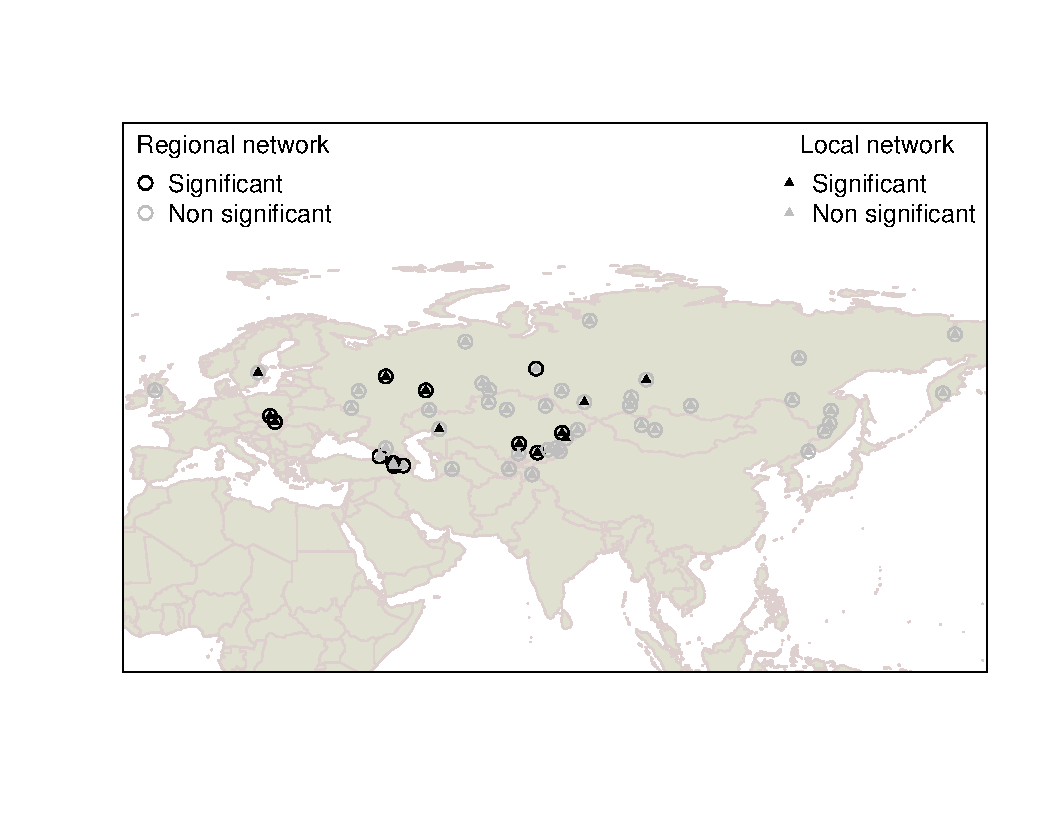
\includegraphics[width=1.00000\textwidth]{figures/figure1.pdf}
\caption{Spatial distribution of co-phylogenetic matching across the 51
sites. For each location, we indicate whether or not the structure of
regional and local interaction networks is consistent with phylogenetic
congruence. The colour of the circle corresponds to regionally
significant or non-significant (black and grey, respectively) while the
colour of the symbol within corresponds to locally significant or
non-significant (black and grey, respectively).\label{fig:maps}}
\end{figure}

\section{Results and discussion}\label{results-and-discussion}

Splitting the datasets at the continental, regional, and local levels
delineates clear quantitative predictions. At the regional scale, one
can expect community assembly to promote the co-occurrence of
evolutionarily linked species pairs -- \emph{i.e.}, a host and a
parasite from lineages that interact will tend to co-occur more often
because the parasites are filtered to be present in sites where they can
find hosts. Under this situation, we expect that regional networks will
have a high degree of phylogenetic matching (because they account for
the information on potential species interactions); we do in addition
expect that their phylogenetic signal will be larger than what is found
in the continental network, since the latter represents a somewhat
artefactual agglomeration of species pairs that do not co-occur. The
opposite situation (a relatively lower phylogenetic matching) would
therefore be suggestive of a weaker selection for the co-occurrence of
evolutionarily tied species pairs.

At the local scale, if interactions between species at matching
phylogenetic positions are conserved, we would expect both a similar or
higher level of phylogenetic matching between the local and the regional
scale, and a positive relationship between the frequency of interaction
and its overall importance for phylogenetic matching (interactions with
a strong phylogenetic signal happen more often). On the contrary, if
local assembly proceeds largely independently from the co-evolutionary
history, the relative level of phylogenetic matching in local networks
should be the same as in the regional networks (through a sampling
effect from the distribution of interaction-level contribution to
cophylogenetic matching), but the frequency of interactions should bear
no relationship to their importance in overall matching.

\subsection{Local and regional scale networks show no co-phylogenetic
matching}\label{local-and-regional-scale-networks-show-no-co-phylogenetic-matching}

As host-macroparasite interactions are hypothesized to be ecologically
constrained, as a result of their being evolutionary conserved (Combes
2001), the congruence observed at the continental level sets the
baseline for what would be expected in local communities. Of course, if
ecological mechanisms (such as filtering) reduce co-phylogenetic
matching, we should detect this signal at the continental scale but not
locally. Out of 51 sites, our \emph{PACo} analysis indicates that 35
show no signal of co-phylogenetic matching at all, 11 show significant
co-phylogenetic matching when using the regional interactions, and 12
show significant co-phylogenetic matching using the local interactions
(see \emph{Supp. Mat. 1} for network-level significance values;
\autoref{maps}). These results support the idea that macro-evolutionary
processes, such as co-diversification, can have consequences at the
macro-ecological level but may not in fact be detectable at finer
spatial scales.

\subsection{Local and regional scale networks have the same relative
co-phylogenetic
matching}\label{local-and-regional-scale-networks-have-the-same-relative-co-phylogenetic-matching}

\begin{figure}[htbp]
\centering
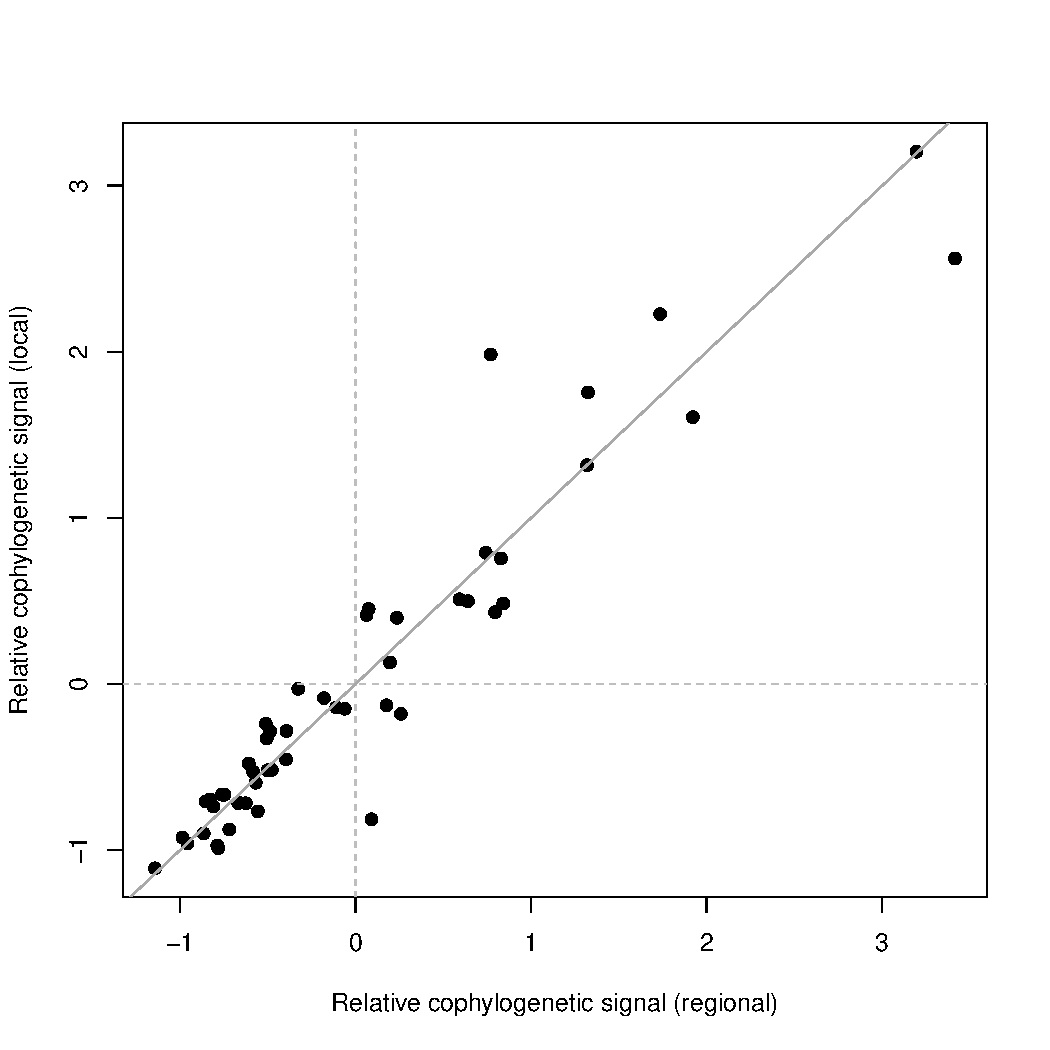
\includegraphics[width=1.00000\textwidth]{figures/figureLocReg.pdf}
\caption{The regional and local networks show the same relative amount
of co-phylogenetic matching. The values presented are the z-scores of
the PACo statistic for the entire network, with the 1:1 relationship
indicated by the solid line.\label{fig:relative}}
\end{figure}

When we compared the relative degree of co-phylogenetic matching in the
local and regional communities (\autoref{relative}), we see that the
relationship between the two is approximately linear (95\% confidence
interval for the correlation coefficient \(0.914\)--\(0.971\)). This
fits with the hypothesis of local networks being assembled by a random
sampling from regional networks: if interactions between species at
matching positions in both trees are maintained by the same set of
drivers, then this should be reflected in the local networks by a higher
degree of cophylogenetic matching.

\subsection{Co-phylogenetic matching is predicted by the contribution of
interactions}\label{co-phylogenetic-matching-is-predicted-by-the-contribution-of-interactions}

\begin{no-prefix-figure-caption}

\begin{figure}[htbp]
\centering
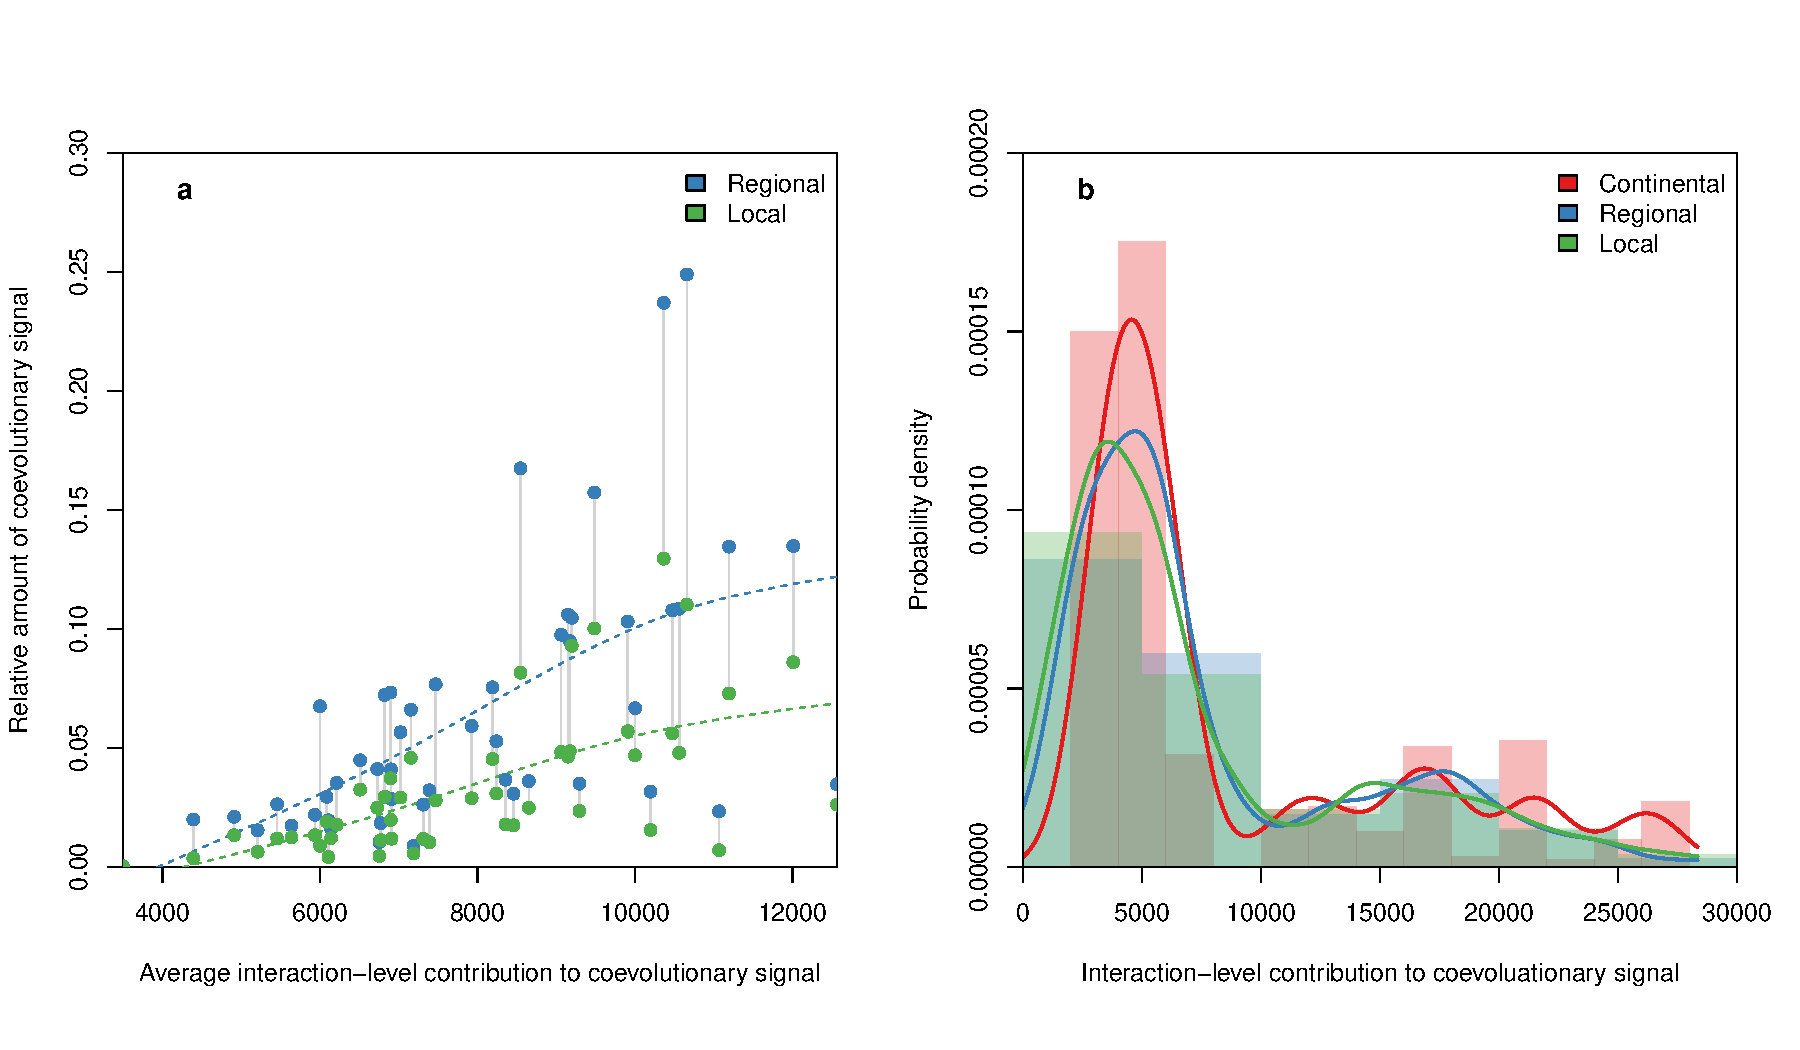
\includegraphics[width=1.00000\textwidth]{figures/figure4.pdf}
\caption{Distribution of co-phylogenetic matching at the network and
interaction levels. \textbf{a}, Networks that have lower co-phylogenetic
matching at the local or regional level are composed of interactions
that on average contribute little to co-phylogenetic matching at the
continental scale. co-phylogenetic matching is presented relatively to
the continental level co-phylogenetic matching. Dashed lines are a cubic
smoothing spline, and the two levels of the same networks are linked by
solid grey lines. \textbf{b}, Overall, interactions observed at the
local, regional, and continental scale have roughly equivalent
contributions to co-phylogenetic matching. Probability density was
smoothed using a Gaussian kernel density estimator. Raw probability
densities are shown as semi-transparent bars.}\label{fg:contributions}
\end{figure}

\end{no-prefix-figure-caption}

On the other hand, system-level differences say little about the
behavior of individual interactions. Despite the fact most
coevolutionary mechanisms act at the interaction level (Thompson 1999),
most \emph{measures} of it are expressed at the community level. We
observe here that networks with interactions that are important for
co-phylogenetic matching at the continental scale are also important for
co-phylogenetic matching at the local and regional scales as well
(\(\rho = 0.95\); \autoref{contributions}A). Intriguingly, we also find
that the distribution of individual interactions' contributions to
co-phylogenetic matching is strongly conserved, regardless of the scale
at which the interactions are quantified (\autoref{contributions}B).
Because interactions differ between each other in terms of their total
contribution to co-phylogenetic matching, this implies that their
distribution across networks (\emph{i.e.} whether the local network
contains a sample of strongly contributing, or weakly contributing,
interactions) is what actually drives differences in overall
co-phylogenetic matching. As such, network-level co-phylogenetic
matching emerges directly from the properties of interactions and is not
a property of the network itself.

\subsection{Interactions contributing to co-phylogenetic matching are
marginally more spatially
consistent}\label{interactions-contributing-to-co-phylogenetic-matching-are-marginally-more-spatially-consistent}

\begin{figure}[htbp]
\centering
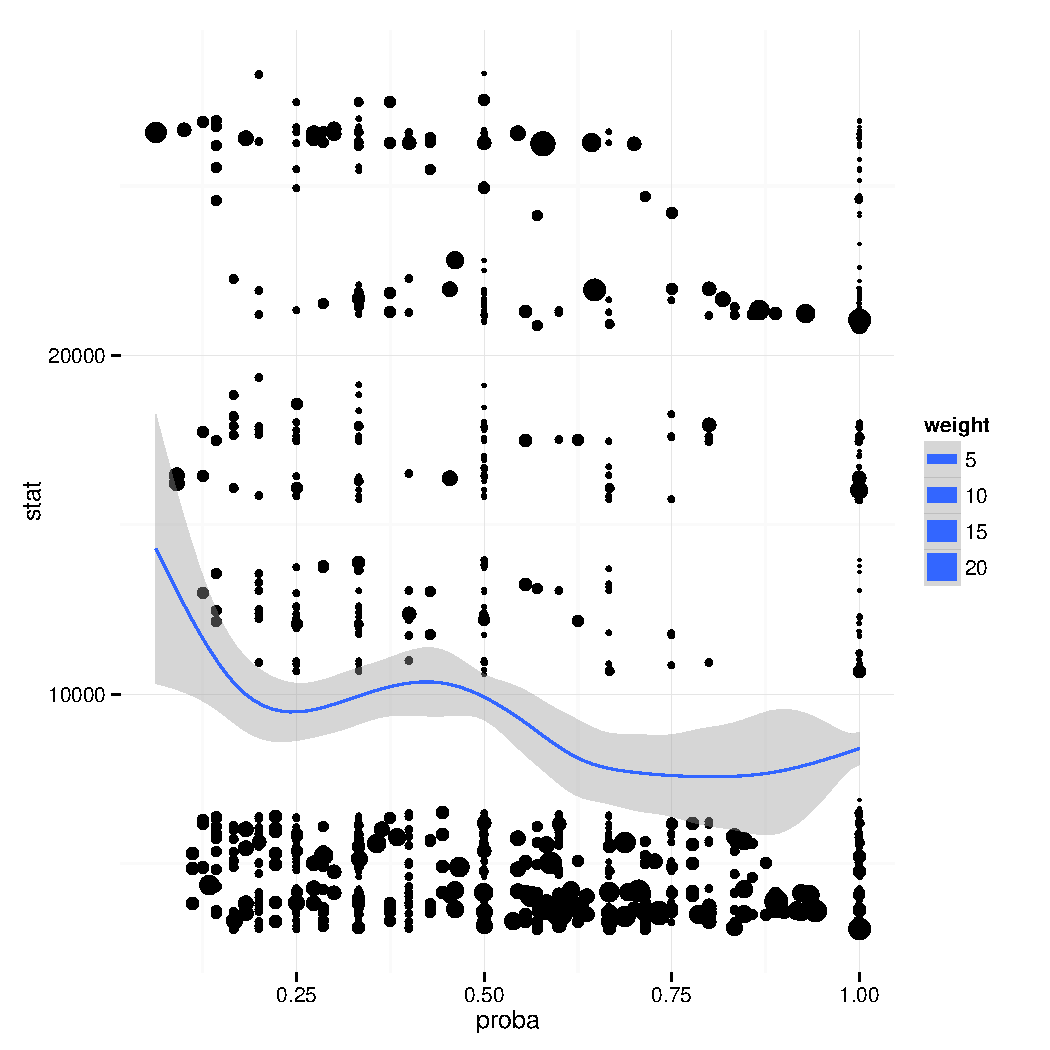
\includegraphics[width=0.80000\textwidth]{figures/figure3.pdf}
\caption{Spatial consistency of an interaction and its contribution to
co-phylogenetic matching. Note that because \emph{PACo} gives low scores
to interactions with a strong contribution to co-phylogenetic matching,
the y axis is reversed. Spatial consistency is defined as the
probability of observing an interaction between two species given that
they were observed to co-occur. Although statistically significant,
there was no biologically meaningful relationship between spatial
consistency and an interaction's importance for co-phylogenetic matching
in the continental network (\(R^2 \approx 0.01\), \(\rho = -0.1\),
\(p \leq 10^{-5}\)).\label{fig:consistency}}
\end{figure}

Beyond their contribution to co-phylogenetic matching, interactions also
ultimately differ in how frequently they vary when the species involved
co-occur (Carstensen et al. 2014; Olito \& Fox 2015; Trøjelsgaard et al.
2015). This can happen, for example, when one of the partners is able to
forage for optimal resources (Betts et al. 2015). Once more, the
literature on host-parasite interactions assumes that the reason why
some interactions are more frequent is because they reflect a
significant past history of coevolution (Guimaraes et al. 2007; 2010);
that is, the ecological constraints emerge from evolutionary
conservatism. Using a weighted Pearson's correlation between the
interaction frequency, interaction contribution to co-phylogenetic
matching, and the number of observations of each interaction as the
weight, we observe that this is marginally true (\(\rho \approx -0.11\).
\(t \approx -5.09\) with weights; \(\rho \approx -0.10\),
\(t \approx -4.6\) without; both significant at \(\alpha = 0.05\);
\autoref{consistency}). Recall that the \emph{negative} correlation here
arises from the fact that high interaction-level values in PACo means
\emph{low} contribution to co-phylogenetic signal. Nevertheless, the
significance of this result ought to be tempered by the fact that the
\(R^2\) of both regressions is close to \(0.01\). Consequently, the
association between spatial consistency and contribution to
co-phylogenetic signal, while statistically significant, explains so
little variance of either quantities that it is likely of negligible
biological importance. This implies that the spatial consistency of an
interaction does not necessarily reflect its evolutionary past, but
rather (possibly) extant ecological processes.

\subsection{The contribution of interactions to co-phylogenetic matching
is consistent across
scales}\label{the-contribution-of-interactions-to-co-phylogenetic-matching-is-consistent-across-scales}

\begin{figure}[htbp]
\centering
\includegraphics[width=1.00000\textwidth]{figures/figure2.pdf}
\caption{The contribution to co-phylogenetic matching of the interaction
between two species is maintained across scales. For every site (ranked
on the x axis), we show the Pearson's correlation between
interaction-level values of co-phylogenetic matching in the continental
network and the same in the local network. The size of each point is
proportional to the size of the network, and correlations for all sites
are significant at \(\alpha = 0.05\) except for those falling in the
grey shaded area.\label{fig:scales}}
\end{figure}

Ultimately, co-phylogenetic matching varies across scale because of the
simultaneous variation of species' interactions \emph{and} communities'
phylogenetic tree structure. In a system characterised by substantial
turnover, we would expect the contribution of each separate interaction
to differ across scales as well. Instead, we observe here that
interactions that contribute strongly to co-phylogenetic matching at the
continental scale \emph{also} show a significant tendency to contribute
strongly at the local (\(p < 0.05\) for positive correlations in 48 out
of 51 networks) and regional (in 47 out of 51 networks), and this
observation is independent of network-wide co-phylogenetic matching
(\autoref{scales}). Remarkably, this result implies that the remnants of
co-phylogenetic inertia are still locally detectable in \emph{individual
interactions} even though shared evolutionary history regularly fails to
leave its imprint on most local networks.

\section{Conclusions}\label{conclusions}

Overall, the results of our study demonstrate that there is a sizeable
gap between our current understanding of host-parasite co-evolution as
the basis of multi-species interactions, its phylogenetic consequences,
and their applicability to ecological questions. Our results suggest
that, while the continental-scale system might show a strong signal of
past coevolution through significantly matching phylogenies (which was
also reported, through different analyses, by other studies of this
system), the quasi-entirety of this signal is lost when species and
their interactions are filtered to assemble local communities. That
there is no further loss of signal from the regional to the local scale
strongly suggests that the loss of signal from the continental to
regional scale is due to species sampling in a manner that proceeds
independently of the evolutionary history of species pairs. Because
regional and local networks have the same species, the difference
between them stems from the loss of some species interactions locally.
It would therefore seem that local species pools in this system are also
driven by the interaction between abiotic conditions and species
tolerance, in addition to potential species interactions. Taking a step
back, this result suggests that while a shared phylogenetic history is a
strong structuring force at the scale of the species pool, its influence
is overridden by other factors during species filtering and community
assembly. This does beg for future investigation of whether the
importance of phylogenetic history decays at smaller spatial scale in
host-parasite assemblages.

Recently, Coelho et al. (2017) studied the factors that shape
phylogenetic signal in bipartite interactions betweeen plants and
mutualists. In contrast to our study, they used a Mantel test to compare
the two trees; this is known to be lacking robustness (Harmon \& Glor
2010; Guillot \& Rousset 2013), which is what originally prompted the
development of PACo (Balbuena et al. 2013) or ParaFit (Legendre et al.
2002). Leaving aside the relative merits of the various methods, they
show that phylogenetic signal is expected to decrease when (1) dispersal
probability increases (\emph{i.e.} all locations share the same species)
and (2) the probability of interactions is high (\emph{i.e.} there is no
loss of signal due to local interaction filtering). We argue that the
probability of interaction should not be viewed as a system-wide
measure, but rather be defined for each interaction
(\xrefname{eq.}\cref{eq:linktunover}). When this is the case, we report
no relationship between the probability of interaction, and its
contribution to phylogenetic signal
(\xrefname{fig.}\cref{fig:consistency}).

Local networks show little to no signal of co-phylogenetic matching, and
the strength of co-phylogenetic matching that can be ascribed to the
interactions between two species is a surprisingly poor predictor of how
frequently they interact. In contrast to the frequent assumption that
phylogenetic structure is a key driver of community structure
(Cavender-Bares et al. 2009), these data reveal that this impact is
actually minimal at ecologically relevant spatial scales. And yet,
despite all the above, individual interactions are somehow able to
maintain their co-phylogenetic matching even when the community they are
woven into does not. Thinking more broadly, these discrepancies provide
a clear roadmap for bridging the gap between our appreciation of the
role of shared evolutionary history and its empirically measurable
outcomes: network structure is the most parsimonious \emph{mechanism} by
which coevolution proceeds, not the imprint potential coevolution leaves
on ecological communities.

\textbf{Acknowledgements.} We thank Juan Antonio Balbuena for
discussions about the \emph{PACo} method, and members of the Stouffer
and Tylianakis groups for comments on an early draft of this manuscript.
We thank Scott Nuismer for feedback. We are indebted to Matt Hutchinson
and Fernando Cagua for contributions to the code of the \lstinline!paco!
R package. Funding to TP and DBS was provided by a Marsden Fund
Fast-Start grant (UOC-1101) and to DBS by a Rutherford Discovery
Fellowship, both administered by the Royal Society of New Zealand.

\section*{References}\label{references}
\addcontentsline{toc}{section}{References}

\hypertarget{refs}{}
\hypertarget{ref-balb13pnp}{}
\textbf{Balbuena et al.} (2013). PACo: A Novel Procrustes Application to
Cophylogenetic Analysis. \emph{PLoS ONE.} 8:e61048.

\hypertarget{ref-benk03rsc}{}
\textbf{Benkman et al.} (2003). Reciprocal selection causes a
coevolutionary arms race between crossbills and lodgepole pine. \emph{Am
Nat.} 162:182--94.

\hypertarget{ref-bett15prk}{}
\textbf{Betts et al.} (2015). Pollinator recognition by a keystone
tropical plant. \emph{Proceedings of the National Academy of Sciences of
the United States of America.} 112:3433--8.

\hypertarget{ref-cana14een}{}
\textbf{Canard et al.} (2014). Empirical evaluation of neutral
interactions in host-parasite networks. \emph{The American Naturalist.}
183:468--79.

\hypertarget{ref-cars14bdp}{}
\textbf{Carstensen et al.} (2014). Beta Diversity of Plant-Pollinator
Networks and the Spatial Turnover of Pairwise Interactions. \emph{PLoS
ONE.} 9:e112903.

\hypertarget{ref-cave09mce}{}
\textbf{Cavender-Bares et al.} (2009). The merging of community ecology
and phylogenetic biology. \emph{Ecol Lett.} 12:693--715.

\hypertarget{ref-coel17nbp}{}
\textbf{Coelho et al.} (2017). Neutral biogeography of phylogenetically
structured interaction networks. \emph{Ecography.}

\hypertarget{ref-comb01pee}{}
\textbf{Combes}. (2001). Parasitism - The Ecology and Evolution of
Intimate Interactions. University Of Chicago Press;

\hypertarget{ref-desd03qps}{}
\textbf{Desdevises et al.} (2003). Quantifying phylogenetically
structured environmental variation. \emph{Evolution.} 57:2647--52.

\hypertarget{ref-dini08mgc}{}
\textbf{Diniz-Filho \& Bini}. (2008). Macroecology, global change and
the shadow of forgotten ancestors. \emph{Glob Ecol Biogeogr.} 17:11--7.

\hypertarget{ref-eklo12reh}{}
\textbf{Eklöf et al.} (2012). Relevance of evolutionary history for food
web structure. \emph{Proceedings of the Royal Society of London B:
Biological Sciences.} 279:1588--96.

\hypertarget{ref-fahr13eua}{}
\textbf{Fahrenholz}. (1913). Ectoparasiten und abstammungslehre.
\emph{Zool Anz.} 41:371--4.

\hypertarget{ref-gale13feb}{}
\textbf{Galetti et al.} (2013). Functional Extinction of Birds Drives
Rapid Evolutionary Changes in Seed Size. \emph{Science.} 340:1086--90.

\hypertarget{ref-gand08hcp}{}
\textbf{Gandon et al.} (2008). Host-parasite coevolution and patterns of
adaptation across time and space. \emph{J Evol Biol.} 21:1861--6.

\hypertarget{ref-guil13dmt}{}
\textbf{Guillot \& Rousset}. (2013). Dismantling the Mantel tests.
Harmon, ed. \emph{Methods in Ecology and Evolution.} 4:336--44.

\hypertarget{ref-guim07iia}{}
\textbf{Guimaraes et al.} (2007). Interaction intimacy affects structure
and coevolutionary dynamics in mutualistic networks. \emph{Curr Biol.}
17:1797--803.

\hypertarget{ref-guim11ecm}{}
\textbf{Guimarães Jr et al.} (2011). Evolution and coevolution in
mutualistic networks. \emph{Ecol Lett.} 14:877--85.

\hypertarget{ref-harm10psp}{}
\textbf{Harmon \& Glor}. (2010). POOR STATISTICAL PERFORMANCE OF THE
MANTEL TEST IN PHYLOGENETIC COMPARATIVE ANALYSES. \emph{Evolution.}

\hypertarget{ref-hemb14cdl}{}
\textbf{Hembry et al.} (2014). Coevolution and the Diversification of
Life. \emph{The American Naturalist.} 184:425--38.

\hypertarget{ref-hutc17pip}{}
\textbf{Hutchinson et al.} (2017). paco: implementing Procrustean
Approach to Cophylogeny in R. \emph{Methods in Ecology and Evolution.}

\hypertarget{ref-john17blc}{}
\textbf{Johnson et al.} (2017). Biodiversity losses and conservation
responses in the Anthropocene. \emph{Science.} 356:270--5.

\hypertarget{ref-jord03ipc}{}
\textbf{Jordano et al.} (2003). Invariant properties in coevolutionary
networks of plant--animal interactions. \emph{Ecology Letters.}
6:69--81.

\hypertarget{ref-kras12psm}{}
\textbf{Krasnov et al.} (2012a). Phylogenetic Signal in Module
Composition and Species Connectivity in Compartmentalized Host-Parasite
Networks. \emph{The American Naturalist.} 179:501--11.

\hypertarget{ref-kras12dfp}{}
\textbf{Krasnov et al.} (2012b). Data from: Phylogenetic signal in
module composition and species connectivity in compartmentalized
host-parasite networks.

\hypertarget{ref-krit91dmh}{}
\textbf{Kritsky}. (1991). Darwin's Madagascan Hawk Moth Prediction.
\emph{American Entomologist.} 37:206--10.

\hypertarget{ref-lege02sth}{}
\textbf{Legendre et al.} (2002). A statistical test for host-parasite
coevolution. \emph{Syst Biol.} 51:217--34.

\hypertarget{ref-mora15ibi}{}
\textbf{Morales-Castilla et al.} (2015). Inferring biotic interactions
from proxies. \emph{Trends in Ecology \& Evolution.}

\hypertarget{ref-mouq12eap}{}
\textbf{Mouquet et al.} (2012). Ecophylogenetics: advances and
perspectives. \emph{Biol Rev.} 87:769--85.

\hypertarget{ref-nuis15pri}{}
\textbf{Nuismer \& Harmon}. (2015). Predicting rates of interspecific
interaction from phylogenetic trees. \emph{Ecol Lett.} 18:17--27.

\hypertarget{ref-nuis13cam}{}
\textbf{Nuismer et al.} (2013). Coevolution and the Architecture of
Mutualistic Networks. \emph{Evolution.} 67:338--54.

\hypertarget{ref-olit15staa}{}
\textbf{Olito \& Fox}. (2015). Species traits and abundances predict
metrics of plant--pollinator network structure, but not pairwise
interactions. \emph{Oikos.} 124:428--36.

\hypertarget{ref-pois152wc}{}
\textbf{Poisot}. (2015). 23 When is co-phylogeny evidence of
coevolution? \emph{Parasite Diversity and Diversification: Evolutionary
Ecology Meets Phylogenetics.}:420.

\hypertarget{ref-pois12dsi}{}
\textbf{Poisot et al.} (2012). The dissimilarity of species interaction
networks. \emph{Ecol Lett.} 15:1353--61.

\hypertarget{ref-pois15swe}{}
\textbf{Poisot et al.} (2015). Beyond species: why ecological
interaction networks vary through space and time. \emph{Oikos.}
124:243--51.

\hypertarget{ref-raff15psf}{}
\textbf{Rafferty et al.} (2015). Phenological shifts and the fate of
mutualisms. \emph{Oikos.} 124:14--21.

\hypertarget{ref-reze07ncp}{}
\textbf{Rezende et al.} (2007). Non-random coextinctions in
phylogenetically structured mutualistic networks. \emph{Nature.}
448:925--8.

\hypertarget{ref-stou12ecs}{}
\textbf{Stouffer et al.} (2012). Evolutionary Conservation of Species'
Roles in Food Webs. \emph{Science.} 335:1489--92.

\hypertarget{ref-thom99rmc}{}
\textbf{Thompson}. (1999). The raw material for coevolution.
\emph{Oikos.} 84:5--16.

\hypertarget{ref-troj15gvm}{}
\textbf{Trøjelsgaard et al.} (2015). Geographical variation in
mutualistic networks: similarity, turnover and partner fidelity.
\emph{Proceedings of the Royal Society B: Biological Sciences.}
282:20142925--5.

\hypertarget{ref-vale10cpr}{}
\textbf{Vale \& Little}. (2010). CRISPR-mediated phage resistance and
the ghost of coevolution past. \emph{Proc R Soc B Biol Sci.}

\hypertarget{ref-van73nel}{}
\textbf{Van Valen}. (1973). A new evolutionary law. \emph{Evol Theory.}
1:1--30.

\hypertarget{ref-vern09lpf}{}
\textbf{Verneau et al.} (2009). Lessons from parasitic flatworms about
evolution and historical biogeography of their vertebrate hosts. \emph{C
R Biol.} 332:149--58.

\hypertarget{ref-mora10bhi}{}
(2010). Biogreography of host-parasite interactions. Morand, Krasnov,
eds. Oxford: Oxford University Press;

\end{document}
